\documentclass[12pt]{article}
\usepackage[utf8]{inputenc}
\usepackage{geometry}
\usepackage{hyperref}
\usepackage{graphicx}
\usepackage{tabularx}
\usepackage{enumitem}
\geometry{a4paper, margin=1in}
\title{\textbf{Settlers of Catan - Guia Estratégico}}
\author{Miguel Cabral Pinto}
\date{}

\begin{document}
\maketitle
\renewcommand{\contentsname}{Índice}
\tableofcontents
\newpage

\section{Introdução}
Fiz este guia para partilhar o meu entendimento do jogo de tabuleiro Settlers of Catan\texttrademark\space com os meus amigos.
Serve de compêndio das informações que reuni através de outros guias estratégicos misturados com o meu próprio conhecimento, e, como tal, é recomendado ter uma noção das regras do jogo antes de o ler, que podem ser consultadas \href{https://colonist.io/catan-rules}{aqui}. 
Finalmente, este documento tem o propósito de ser melhorado ao longo do tempo, por isso sente-te à vontade para me dar qualquer tipo de sugestões!

\section{Fundamentos}

\subsection{Recursos}
\begin{tabularx}{\textwidth}{|p{0.14\textwidth}|p{0.08\textwidth}|X|p{0.08\textwidth}|}
    \hline
    \textbf{Recurso} & \textbf{Uso} & \textbf{Valor} & \textbf{Hexs} \\
    \hline
    \raisebox{-0.5\height}{
\includegraphics[height=10pt]{../imgs/wood.png} \textbf{Wood}} & \raisebox{-0.5\height}{
\includegraphics[height=10pt]{../imgs/settle.png} 
\includegraphics[height=10pt]{../imgs/road.png}} & Valor acrescido no início do jogo, e para estratégias de Longest Road. & 4 \\
    \hline
    \raisebox{-0.5\height}{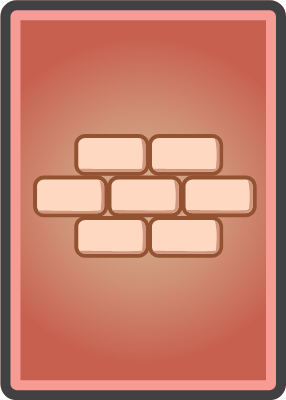
\includegraphics[height=10pt]{../imgs/brick.png} \textbf{Brick}} & \raisebox{-0.5\height}{
\includegraphics[height=10pt]{../imgs/settle.png} 
\includegraphics[height=10pt]{../imgs/road.png}} & Como \raisebox{-0.15\height}{
\includegraphics[height=10pt]{../imgs/wood.png}}, mas mais escasso, por isso tendencialmente mais valioso. & 3 \\
    \hline
    \raisebox{-0.5\height}{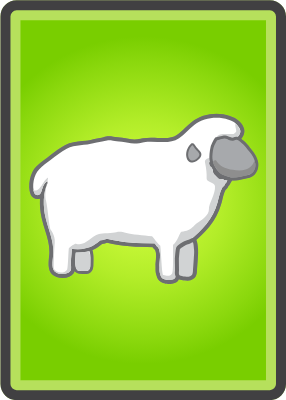
\includegraphics[height=10pt]{../imgs/sheep.png} \textbf{Sheep}} & \raisebox{-0.5\height}{
\includegraphics[height=10pt]{../imgs/settle.png} 
\includegraphics[height=10pt]{../imgs/dev.png}} & Valor moderado, mas é sempre preciso um pouco para qualquer estratégia, especialmente se passar por comprar \raisebox{-0.15\height}{
\includegraphics[height=10pt]{../imgs/dev.png}}. & 4 \\
    \hline
    \raisebox{-0.5\height}{
\includegraphics[height=10pt]{../imgs/wheat.png} \textbf{Wheat}} & \raisebox{-0.5\height}{
\includegraphics[height=10pt]{../imgs/settle.png} 
\includegraphics[height=10pt]{../imgs/city.png} 
\includegraphics[height=10pt]{../imgs/dev.png}} & Muito valioso durante todo o jogo, dado que é preciso para fazer praticamente tudo. & 4 \\
    \hline
    \raisebox{-0.5\height}{
\includegraphics[height=10pt]{../imgs/ore.png} \textbf{Ore}} & \raisebox{-0.5\height}{
\includegraphics[height=10pt]{../imgs/city.png} 
\includegraphics[height=10pt]{../imgs/dev.png}} & Muito valioso, especialmente para o final do jogo, no qual \raisebox{-0.1\height}{
\includegraphics[height=10pt]{../imgs/city.png}} são a melhor forma de aumentar a produção. & 3 \\
    \hline
\end{tabularx}

\subsection{Compras}
\begin{tabularx}{\textwidth}{|p{0.15\textwidth}|p{0.12\textwidth}|X|p{0.07\textwidth}|}
    \hline
    \textbf{Compra} & \textbf{Custo} & \textbf{Benefício} & \textbf{VPs} \\
    \hline
    \raisebox{-0.5\height}{
\includegraphics[height=10pt]{../imgs/road.png} \textbf{Road}} & \raisebox{-0.5\height}{
\includegraphics[height=10pt]{../imgs/wood.png} 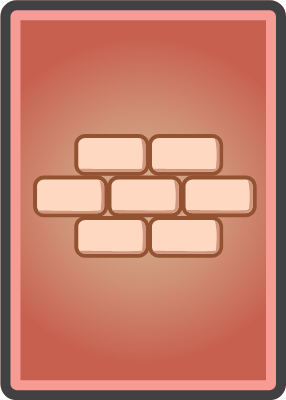
\includegraphics[height=10pt]{../imgs/brick.png}} & Expande a rede de \raisebox{-0.1\height}{
\includegraphics[height=10pt]{../imgs/settle.png}} posicionáveis e pode contribuir para Longest Road. & 0 \\
    \hline
    \raisebox{-0.5\height}{
\includegraphics[height=10pt]{../imgs/settle.png} \textbf{Settle}} & \raisebox{-0.5\height}{
\includegraphics[height=10pt]{../imgs/wood.png} 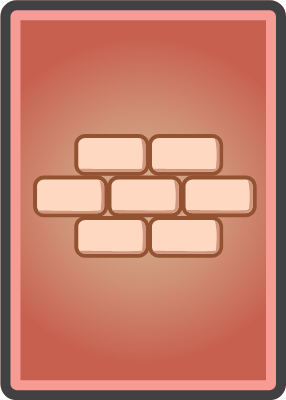
\includegraphics[height=10pt]{../imgs/brick.png} 
\includegraphics[height=10pt]{../imgs/wheat.png} 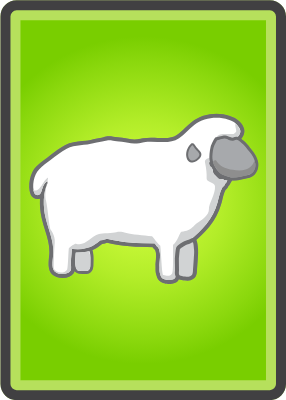
\includegraphics[height=10pt]{../imgs/sheep.png}} & Garante recursos ao utilizador se calhar o número dos hexágonos adjacentes. Forma mais utilizada de aumentar a produção no início do jogo, de modo a tomar o máximo de espaço possível. Tem de ter 2 espaços de distância de outras \raisebox{-0.1\height}{
\includegraphics[height=10pt]{../imgs/settle.png}}. & 1 \\
    \hline
    \raisebox{-0.5\height}{
\includegraphics[height=10pt]{../imgs/city.png} \textbf{City}} & \raisebox{-0.5\height}{
\includegraphics[height=10pt]{../imgs/ore.png} 
\includegraphics[height=10pt]{../imgs/ore.png} 
\includegraphics[height=10pt]{../imgs/ore.png} 
\includegraphics[height=10pt]{../imgs/wheat.png} 
\includegraphics[height=10pt]{../imgs/wheat.png}} & Duplica a produção de recursos de uma \raisebox{-0.1\height}{
\includegraphics[height=10pt]{../imgs/settle.png}}. No final do jogo, torna-se a única forma de melhorar a produção, mas se for construida no início pode ser muito forte. & 2 \\
    \hline
    \raisebox{-0.5\height}{
\includegraphics[height=10pt]{../imgs/dev.png} \textbf{Dev Card}} & \raisebox{-0.5\height}{
\includegraphics[height=10pt]{../imgs/ore.png} 
\includegraphics[height=10pt]{../imgs/wheat.png} 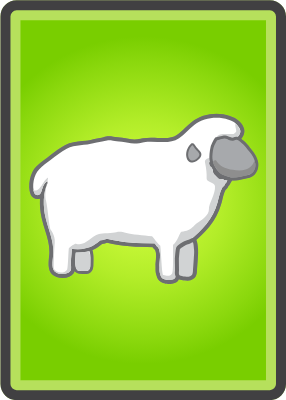
\includegraphics[height=10pt]{../imgs/sheep.png}} & Carta mistério que pode contribuir para ambos os marcos e conter VPs e habilidades úteis. & Var. \\
    \hline
\end{tabularx}

% \subsection{Marcos}
% \begin{tabularx}{\textwidth}{|p{0.21\textwidth}|X|}
%     \hline
%     \textbf{Marco} & \textbf{Descrição} \\
%     \hline
%     \raisebox{-0.5\height}{\raisebox{-0.15\height}{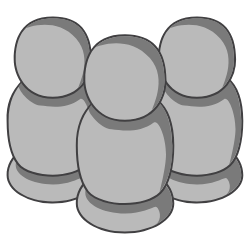
\includegraphics[height=10pt]{../imgs/army.png}} \textbf{Largest Army}} & O primeiro jogador a chegar ao número máximo atual de \raisebox{-0.15\height}{
\includegraphics[height=10pt]{../imgs/knight.png}} usados superior a 3 recebe 2 VPs.\\
%     \hline
%     \raisebox{-0.5\height}{\raisebox{-0.15\height}{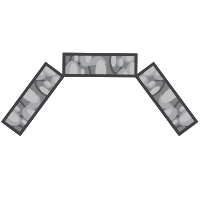
\includegraphics[height=10pt]{../imgs/longest_road.png}} \textbf{Longest Road}} & O primeiro jogador a ter a maior sequência atual de \raisebox{-0.15\height}{
\includegraphics[height=10pt]{../imgs/road.png}} consecutivas superior a 5 recebe 2 VPs.\\
%     \hline
% \end{tabularx}

\subsection{Cartas de Desenvolvimento}
\begin{tabularx}{\textwidth}{|p{0.16\textwidth}|X|}
    \hline
    \textbf{Carta} & \textbf{Benefício} \\
    \hline
    \raisebox{-0.5\height}{
\includegraphics[height=10pt]{../imgs/knight.png} \textbf{Knight}} & Quando jogada, permite ao utilizador posicionar o Robber e roubar uma carta aleatória a um jogador bloqueado. Usos incluem remover o Robber de um hexágono de interesse, abrandar adversários bloqueando-os e contribuir para Largest Army. \\
    \hline
    \raisebox{-0.5\height}{
\includegraphics[height=10pt]{../imgs/vp.png} \textbf{VP}} & Quando comprada, dá ao proprietário um VP escondido. A sua posse deve ser ocultada o máximo de tempo possível, para que a pontuação real do jogador se mantenha um mistério para os outros. \\
    \hline
    \raisebox{-0.5\height}{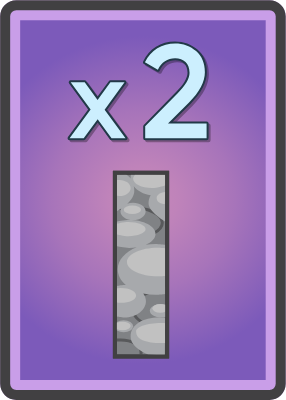
\includegraphics[height=10pt]{../imgs/road_building.png} \textbf{Road}} \newline \raisebox{-0.5\height}{\textbf{Building}} & Quando jogada, o utilizador pode construir 2 \raisebox{-0.15\height}{
\includegraphics[height=10pt]{../imgs/road.png}} ligadas à sua rede. Muito útil no início do jogo para deslocamento no tabuleiro sem gastar \raisebox{-0.15\height}{
\includegraphics[height=10pt]{../imgs/wood.png} 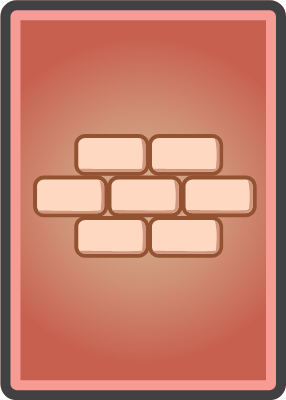
\includegraphics[height=10pt]{../imgs/brick.png}}, facilitando o estabelecimento de \raisebox{-0.1\height}{\includegraphics[height=10pt]{../imgs/settle.png}}. Contribui também para Longest Road.\\
    \hline
    \raisebox{-0.5\height}{\includegraphics[height=10pt]{../imgs/yop.png} \textbf{Year}} \newline \raisebox{-0.5\height}{\textbf{of Plenty}} & Quando jogada, o utilizador escolhe 2 cartas de recurso do banco. Deve ser usada para receber recursos não produzidos ou para concluir um projeto para o qual faltam cartas. (Ex: \raisebox{-0.15\height}{\includegraphics[height=10pt]{../imgs/wheat.png} \includegraphics[height=10pt]{../imgs/wheat.png} \includegraphics[height=10pt]{../imgs/ore.png}} + (\raisebox{-0.15\height}{\includegraphics[height=10pt]{../imgs/yop.png}} $\rightarrow$ \raisebox{-0.15\height}{\includegraphics[height=10pt]{../imgs/ore.png} \includegraphics[height=10pt]{../imgs/ore.png}}) = \raisebox{-0.1\height}{\includegraphics[height=10pt]{../imgs/city.png}})\\
    \hline
    \raisebox{-0.5\height}{\includegraphics[height=10pt]{../imgs/mono.png} \textbf{Monopoly}} & Quando jogada, o utilizador rouba todas as cartas de um recurso específico dos baralhos dos outros jogadores. Considerada muita forte pelo seu potencial de controlar o supply de um certo recurso e excelente sinergia com portos. \textit{``You should always try to get at least 2 points from a \raisebox{-0.15\height}{\includegraphics[height=10pt]{../imgs/mono.png}}!''} - DandyDrew (Rei do Catan)\\
    \hline
\end{tabularx}

\section{Estratégias}

\begin{itemize}
    \item \textbf{OWS $\rightarrow$}
    Recursos iniciais: \raisebox{-0.15\height}{\includegraphics[height=10pt]{../imgs/sheep.png} \includegraphics[height=10pt]{../imgs/wheat.png} \includegraphics[height=10pt]{../imgs/ore.png}}.
    Foco em Largest Army.
    Os recursos escolhidos inicialmente permitem investimento rápido em \raisebox{-0.1\height}{\includegraphics[height=10pt]{../imgs/city.png}} e \raisebox{-0.15\height}{\includegraphics[height=10pt]{../imgs/dev.png}}, dependendo de trocas com o banco e/ou outros jogadores para obter \raisebox{-0.15\height}{\includegraphics[height=10pt]{../imgs/wood.png} \includegraphics[height=10pt]{../imgs/brick.png}} necessários para assegurar a mobilidade mínima. 
    Ao ultrapassar esta dificuldade e construir \raisebox{-0.1\height}{\includegraphics[height=10pt]{../imgs/settle.png}}, pode ser muito forte, porque permite que os objetivos mais difíceis do jogo sejam adiantados no início.
    \item \textbf{OWS Híbrido $\rightarrow$}
    Recursos iniciais: \raisebox{-0.15\height}{\includegraphics[height=10pt]{../imgs/sheep.png} \includegraphics[height=10pt]{../imgs/wheat.png} \includegraphics[height=10pt]{../imgs/ore.png}} (\raisebox{-0.15\height}{\includegraphics[height=10pt]{../imgs/wood.png}} \raisebox{-0.15\height}{\includegraphics[height=10pt]{../imgs/brick.png}}).
    Foco em Largest Army.
    Combina a estratégia anterior com \raisebox{-0.15\height}{\includegraphics[height=10pt]{../imgs/wood.png}} ou \raisebox{-0.15\height}{\includegraphics[height=10pt]{../imgs/brick.png}}, trocando um pouco da produção de recursos OWS por flexibilidade. 
    Na maioria dos casos, um OWS puro é inviável pela escassez de bons posicionamentos iniciais, pelo que este poderá ser o mais próximo possível.
    \item \textbf{Road $\rightarrow$}
    Recursos iniciais: \raisebox{-0.15\height}{\includegraphics[height=10pt]{../imgs/wood.png} \includegraphics[height=10pt]{../imgs/brick.png}} (\raisebox{-0.15\height}{\includegraphics[height=10pt]{../imgs/sheep.png} \includegraphics[height=10pt]{../imgs/wheat.png} \includegraphics[height=10pt]{../imgs/ore.png}}).
    Foco em Longest Road.
    Prioriza uma expansão rápida no início do jogo, dado que o controlo de uma porção do tabuleiro facilita muito o objetivo desta estratégia, para além de permitir a construção de \raisebox{-0.1\height}{\includegraphics[height=10pt]{../imgs/settle.png}}.
    \item \textbf{City + Road $\rightarrow$}
    Recursos iniciais: \raisebox{-0.15\height}{\includegraphics[height=10pt]{../imgs/wood.png} \includegraphics[height=10pt]{../imgs/brick.png} \includegraphics[height=10pt]{../imgs/wheat.png} \includegraphics[height=10pt]{../imgs/ore.png}}.
    Foco em Longest Road.
    Comparado com \textbf{Road}, equilibra o investimento inicial de modo a permitir a construção de \raisebox{-0.1\height}{\includegraphics[height=10pt]{../imgs/city.png}}, sendo muito flexível por ter outro meio de ganhar pontos e aumentar a produção.
    \item \textbf{5 Recursos $\rightarrow$}
    Recursos iniciais: \raisebox{-0.15\height}{\includegraphics[height=10pt]{../imgs/wood.png} \includegraphics[height=10pt]{../imgs/brick.png} \includegraphics[height=10pt]{../imgs/sheep.png} \includegraphics[height=10pt]{../imgs/wheat.png} \includegraphics[height=10pt]{../imgs/ore.png}}.
    Foco geral.
    Flexibilidade máxima!
    \item \textbf{Porto $\rightarrow$}
    Recursos iniciais: (\raisebox{-0.15\height}{\includegraphics[height=10pt]{../imgs/wood.png} \includegraphics[height=10pt]{../imgs/brick.png} \includegraphics[height=10pt]{../imgs/sheep.png} \includegraphics[height=10pt]{../imgs/wheat.png} \includegraphics[height=10pt]{../imgs/ore.png}}).
    Foco geral.
    Ocorre quando se tem acesso a muito de um recurso específico e ao porto 2:1 correspondente, que se torna o método principal de obter os restantes. 
    Alto potencial, porque o sucesso depende da probabilidade de produzir um só recurso, pelo que se deve aumentá-la ao máximo. 
    Ao alcançar um monopólio, os outros jogadores são forçados a trocar connosco.
\end{itemize}

\section{Fases do Jogo}
\subsection{Posicionamentos Iniciais}
Esta fase determina o desenrolar do jogo, porque as escolhas feitas por cada jogador vão condicionar a sua estratégia (\textit{``You can't win the game with placements, but you can definitely lose it.''} - Treeckosaurus).
É importante analisar a nossa situação (\textbf{disposição do tabuleiro} e \textbf{ordem de posicionamento}) e compará-la com a dos oponentes, de modo a prever quais vão ser as suas escolhas iniciais e fazer as nossas em função disso. \\
Ao começar um jogo, deve-se identificar imediatamente quais os sítios com mais produção no tabuleiro (mais de 10 \raisebox{0.2\height}{\textbullet}), e, desses, quais os que apresentam maior flexibilidade (diversidade de recursos, portos úteis, garantia de boas 2ª escolhas, parceiros potenciais de troca, etc.), o que vai permitir ter uma boa ideia de quais deles vão ser escolhidos.
Dada a disposição vai-vem da ordem de posicionamento, a posição atribuída dita as prioridades:
\begin{itemize}
    \item Quanto mais cedo a 1ª escolha, mais importante é prever corretamente qual vai ser o estado do tabuleiro na 2ª escolha, para maximizar o potencial da nossa estratégia e condicionar a dos outros jogadores.
    No geral, as primeiras \raisebox{-0.10\height}{\includegraphics[height=10pt]{../imgs/settle.png}} são as mais poderosas, porque têm a melhor oportunidade de ficar em bons lugares e monopolizar recursos raros;
    as últimas tendem a ser as menos poderosas e/ou servir para complementar a estratégia escolhida (muito frequentemente, pode ser útil escolher uma posição costal, se tiver boa produção e/ou flexibilidade, como um porto útil).
    \item Quanto mais tarde a 1ª escolha, mais convém ser reativo e adaptar a estratégia às posições dos outros jogadores, procurando condicionar as suas 2ª escolhas.
    Dada a maior proximidade temporal entre os 2 posicionamentos, é mais fácil que estes criem um plano de jogo coeso, mesmo se as melhores posições já tiverem sido ocupadas.
\end{itemize}
É também importante a direção da estrada, especialmente quando se quer uma \raisebox{-0.1\height}{\includegraphics[height=10pt]{../imgs/settle.png}} num lugar contestado ou se tem baixa produção de \raisebox{-0.15\height}{\includegraphics[height=10pt]{../imgs/wood.png} \includegraphics[height=10pt]{../imgs/brick.png}}. 
Ao fazer a escolha, convém pesar a atratividade dos lugares a que esta dá acesso com a probabilidade de lá chegar antes dos outros.
Corridas podem-se resolver fazendo acordos ou até fazendo um \textit{plow} (bloquear a expansão do oponente com uma \raisebox{-0.15\height}{\includegraphics[height=10pt]{../imgs/road.png}}; no geral, ajuda receber \raisebox{-0.15\height}{\includegraphics[height=10pt]{../imgs/wood.png} \includegraphics[height=10pt]{../imgs/brick.png}} como recursos iniciais).

\vspace{-0.1cm}
\subsubsection{Exemplo}

\vspace{-0.5cm}
\begin{figure}[h]
    \begin{minipage}{0.45\textwidth}
        \centering
        \includegraphics[width=\textwidth]{../imgs/example_board_1.png}
        \label{fig:example_board_1}
    \end{minipage}
    \hfill
    \begin{minipage}{0.5\textwidth}
        \raggedright
            Neste tabuleiro, quais os sítios com maior produção? \\
            \textit{\textbf{5-9-10}, \textbf{8-4-10}, \textbf{6-9-3}, \textbf{8-5-10}, \textbf{8-4-3}, \textbf{6-5-11}} \\
            \vspace{0.5cm}

            Quais são os sítios com maior flexibilidade? \\
            \textit{\textbf{5-9-10} tem diversidade e 3:1s, 
            \textbf{6-9-3} tem diversidade e 3:1s, 
            \textbf{8-5-10} tem diversidade e 2:1s úteis} \\
            \vspace{0.5cm}

            Então qual deve ser a 1ª escolha? 
            \vspace{0.5cm}
    \end{minipage}
\end{figure}
\noindent\begin{tabularx}{\textwidth}{|p{0.025\textwidth}|p{0.288\textwidth}|p{0.288\textwidth}|p{0.288\textwidth}|}
    \hline
    \textbf{\#} & \textbf{Cenário 1} & \textbf{Cenário 2} & \textbf{Cenário 3} \\
    \hline
    1 & 
    \textbf{8-5-10}, lugar com alta produção e flexibilidade & 
    \textbf{5-9-10}, lugar com alta produção e flexibilidade & 
    \textbf{6-9-3}, lugar com alta produção e flexibilidade \\
    \hline
    2 & 
    \textbf{5-9-10}, é semelhante à primeira escolha & 
    \textbf{8-5-10}, é semelhante à primeira escolha & 
    \textbf{8-5-10}, lugar com alta produção e flexibilidade \\
    \hline
    3 & 
    \textbf{6-5-11}, é o único bom lugar com \raisebox{-0.15\height}{\includegraphics[height=10pt]{../imgs/wheat.png}} restante e vai ter acesso a \raisebox{-0.15\height}{\includegraphics[height=10pt]{../imgs/ore.png}} na volta & 
    \textbf{6-5-11}, é o único bom lugar com \raisebox{-0.15\height}{\includegraphics[height=10pt]{../imgs/wheat.png}} restante e vai ter acesso a \raisebox{-0.15\height}{\includegraphics[height=10pt]{../imgs/ore.png}} na volta & 
    \textbf{8-4-3}, é o único bom lugar com \raisebox{-0.15\height}{\includegraphics[height=10pt]{../imgs/ore.png}} restante e vai ter acesso a \raisebox{-0.15\height}{\includegraphics[height=10pt]{../imgs/wheat.png}} na volta\\
    \hline
    4 & 
    \textbf{8-4-10}, porque ninguém tem setup para Longest Road e há muito \raisebox{-0.15\height}{\includegraphics[height=10pt]{../imgs/sheep.png} \includegraphics[height=10pt]{../imgs/wheat.png}} no tabuleiro para receber em trocas & 
    \textbf{8-4-10}, porque ninguém tem setup para Longest Road e há muito \raisebox{-0.15\height}{\includegraphics[height=10pt]{../imgs/sheep.png} \includegraphics[height=10pt]{../imgs/wheat.png}} no tabuleiro para receber em trocas & 
    \textbf{6-5-11}, (ver próximo) \\
    \hline
    4 & 
    \textbf{6-9-3}, complementando a estratégia e recebendo o recurso menos produzido (\raisebox{-0.15\height}{\includegraphics[height=10pt]{../imgs/ore.png}}) como inicial & 
    \textbf{6-9-3}, complementando a estratégia e recebendo o recurso menos produzido (\raisebox{-0.15\height}{\includegraphics[height=10pt]{../imgs/ore.png}}) como inicial & 
    \textbf{8-4-10}, assegurando um setup para construir \raisebox{-0.10\height}{\includegraphics[height=10pt]{../imgs/settle.png}} e obter Longest Road com alta produção e \raisebox{-0.15\height}{\includegraphics[height=10pt]{../imgs/road.png}} inicial\\
    \hline
    3 & 
    \textbf{8-4-3}, garantindo OWS puro & 
    \textbf{8-4-3}, garantindo OWS puro & 
    \textbf{5-9-10}, obtendo OWS com um pouco de \raisebox{-0.15\height}{\includegraphics[height=10pt]{../imgs/wood.png}} \\
    \hline
    2 & 
    \textbf{9-4-11}, para ter todos os recursos bem equilibrados e tirar o lugar ao \#1 & 
    \textbf{9-4-11}, mas a diferença de 1ª escolha torna este cenário muito mais favorável (melhor equilíbrio e prob. de chegar aos lugares de 3 hexs restantes) & 
    \textbf{9-4-11}, obtendo o mesmo setup do cenário anterior \\
    \hline
    1 & 
    \textbf{6-3-11}, é o lugar restante com melhor produção e permite dominar o canto superior esquerdo & 
    \textbf{6-3-11}, fica com pior equilíbrio de recursos comparado com o \#2; exemplo de como pequenas escolhas mudam jogos & 
    \textbf{10-3-11}, ficando com um setup que tem um equilíbrio de recursos medíocre e pouca especialização \\
    \hline
\end{tabularx} \\

\noindent Estes cenários servem para ilustrar como a ordem de posicionamento e as escolhas iniciais condicionam o jogo, e como é importante prever as escolhas dos outros jogadores para maximizar o potencial da nossa estratégia.
Não é uma ciência exata nem é trivial de calcular inicialmente, mas ao adquirir experiência torna-se mais natural olhar para o tabuleiro desta forma.

\subsection{Early Game}
O foco principal deve ser em aumentar a produção e a flexibilidade (dependendo da estratégia, pode ser mais fácil fazer isto através de \raisebox{-0.1\height}{\includegraphics[height=10pt]{../imgs/settle.png}} ou \raisebox{-0.1\height}{\includegraphics[height=10pt]{../imgs/city.png}}), adiantar o objetivo de 2 pontos (Longest Road / Largest Army) e completar o nosso desafio mais difícil / importante, como por exemplo construir \raisebox{-0.1\height}{\includegraphics[height=10pt]{../imgs/settle.png}} para estratégias com pouca produção de \raisebox{-0.15\height}{\includegraphics[height=10pt]{../imgs/wood.png} \includegraphics[height=10pt]{../imgs/brick.png}}.
Estes recursos têm valor acrescido no início do jogo, porque ainda há muito espaço para explorar no tabuleiro, em contraste com as próximas fases.
Como regra geral, no final desta fase deve-se ter aumentado significativamente a produção ($>$1.5x), completado a tarefa mais difícil, não estar dependente de trocas 4:1 e ter um plano para chegar aos 10 pontos.

\subsection{Mid Game}
Os oponentes com o melhor início e/ou rivais de estratégia deverão começar a ser bloqueados quando existe essa oportunidade, e os mais atrás podem ser ajudados de modo a equilibrar o jogo. 
Para se ser bloqueado o mínimo possível, é importante o conceito de \textit{pacing}, que é a capacidade de manter um ritmo de desenvolvimento discreto e não chamar a atenção dos outros durante o máximo de tempo possível (é um equilíbrio; não se deve atrasar o desenvolvimento significativamente).
Adicionalmente, jogadores com estratégias de foco geral podem também adaptar o seu plano de jogo em função de como os outros se estão a sair (por exemplo, se o jogador de OWS ainda não tiver comprado \raisebox{-0.15\height}{\includegraphics[height=10pt]{../imgs/dev.png}}, qualquer um pode ficar com Largest Army).

\subsection{End Game}
Começa quando um jogador está muito perto (a menos de 10 cartas) de ganhar o jogo. 
Durante o mid game, deve-se preparar para esta etapa analisando os caminhos dos oponentes para a vitória e escolhendo o nosso de modo a dificultar o deles (por exemplo, se Longest Road é importante para a vitória do oponente mais avançado, tomá-la no fim do jogo pode apanhá-lo de surpresa).

\section{Dicas Avançadas}
\subsection{Trocas}
Trocar é essencial para avançar no jogo, especialmente no early game, em que é a forma claramente mais barata de obter recursos que não se produz.
Deve-se fazer sempre por tentar melhorar o nosso deque de recursos, e, por isso, faz sentido propor trocas em quase todas as jogadas.
Para assegurar a melhor taxa de sucesso possível, é importante praticar \textit{table awareness}, que é a capacidade de perceber o estado do jogo e adaptar a proposta de troca em sua função. 
Incluir monitorizar vários fatores, como:
\vspace{-0.2cm}
\begin{itemize}[noitemsep]
    \item Quem está mais avançado / atrás no jogo?
    \item Que recursos / \raisebox{-0.15\height}{\includegraphics[height=10pt]{../imgs/dev.png}} têm os outros jogadores?
    \item Quais os próximos objetivos de cada jogador?
    \item Quão valiosos são os recursos envolvidos na troca?
\end{itemize}
\vspace{-0.2cm}
Automatizar este tipo de pensamento permite pensar mais rapidamente sobre a viabilidade e valor de uma troca, o que, para trocas recebidas, pode ser a diferença entre escolherem trocar connosco ou não.
Neste sentido, também ajuda prepararmo-nos e estarmos atentos durante as jogadas dos adversários. \\
Outra tática a ter em mente é \textit{open trading}, ao colocar o enfâse no recurso que se pretende dar e não no que se quer receber (\textit{``O que estão dispostos a dar por \raisebox{-0.15\height}{\includegraphics[height=10pt]{../imgs/brick.png}}?''}).
Esta forma de colocar a questão dá menos informação de intenção ao oponente, e pode-se até obter as trocas desejadas sem ter de as pedir explicitamente. \\
Uma última forma criativa de trocar é através de promessas futuras, que são acordos informais que se fazem com outros jogadores ao lhes garantir benefícios no futuro, como o próximo recurso de um certo tipo que recebermos ou um \textit{non-block}/\textit{non-steal} (descritos na secção 8).

\subsection{Uso do Robber}
Normalmente, ao calhar um 7 ou ao jogar um \raisebox{-0.15\height}{\includegraphics[height=10pt]{../imgs/knight.png}}, é boa ideia usar o Robber para bloquear:
\vspace{-0.6cm}
\begin{itemize}[noitemsep]
    \item Hexágonos estratégicos (altamente úteis no momento; frequentemente, \raisebox{-0.15\height}{\includegraphics[height=10pt]{../imgs/wheat.png} \includegraphics[height=10pt]{../imgs/ore.png}} e/ou alta produção são a melhor opção) ao jogador mais à frente / rival de estratégia;
    \item Hexágonos com produção alta de um recurso que já se produz em grandes quantidades, de modo a criar um monopólio e forçar os outros jogadores a fazerem trocas favoráveis connosco;
    \item Jogadores com muitas \raisebox{-0.15\height}{\includegraphics[height=10pt]{../imgs/dev.png}} no seu baralho, obrigando-os a jogar \raisebox{-0.15\height}{\includegraphics[height=10pt]{../imgs/knight.png}} defensivamente, o que dá informação valiosa (se eles não jogarem \raisebox{-0.15\height}{\includegraphics[height=10pt]{../imgs/knight.png}}, é provável terem outras cartas).
\end{itemize}
\vspace{-0.1cm}
No entanto, é preciso encontrar um equilíbrio entre mover o Robber para o melhor sítio estratégico e não fazer demasiados \textit{solo blocks} ou bloqueios repetidos ao mesmo jogador, sendo importante preservar a diplomacia (particularmente no início do jogo). \\
Finalmente, o Robber tem também a funcionalidade de roubar uma carta aleatória a um jogador bloqueado, que é útil para tentar roubar recursos que nos faltam para completar um objetivo ou para roubar recursos que sabemos serem valiosos para o oponente.
Para isto, convém ter uma boa ideia dos recursos possuídos por cada oponente, o que pode ser alcançado através de \textit{tracking}.

\subsection{Tracking}
Pode ser descrita como a prática de monitorizar e/ou prever as cartas que os outros jogadores têm no seu baralho.
\begin{itemize}
    \item Quanto aos recursos, pode ser muito difícil lembrar todas as cartas que os outros jogadores têm, pelo que se torna necessário arranjar formas de simplificar o processo.
    De modo a começar da forma menos complicada possível, pode-se tentar monitorizar apenas um baralho ou a distribuição de um recurso específico.
    Outra forma passa por memorizar os valores do dado em cada ronda, tornando-se apenas necessário associá-los aos respetivos recursos/jogadores.
    Deve-se estar especialmente atento aos valores de que os outros jogadores necessitam para completar o seu próximo objetivo, e também decorar os gastos de cada um.
    Dois desafios nesta prática são:
    \vspace{-0.3cm}
    \begin{itemize}[noitemsep]
        \item Os roubos entre dois oponentes, que são a maior fonte de entropia por passarem uma carta aleatória do baralho de um para outro. 
        É necessário avaliar as probabilidades com base no nosso conhecimento de cada baralho e observar os movimentos de ambos os jogadores para deduzir qual foi o recurso.
        \item Perder conta dos recursos que os outros jogadores têm, podendo-se recomeçar a contagem ao pensar sobre quais os valores que nos concederam os nossos recursos mais recentes e daí inferir os dos oponentes.
    \end{itemize}
    \item Quanto a \raisebox{-0.15\height}{\includegraphics[height=10pt]{../imgs/dev.png}}, para além do método discutido na secção anterior para forçar \raisebox{-0.15\height}{\includegraphics[height=10pt]{../imgs/knight.png}} defensivos, há alguns outros truques que têm em conta o comportamento do jogador:
    \vspace{-0.8cm}
    \begin{itemize}[noitemsep]
        \item Se este pedir recursos para um objetivo para o qual lhe faltam bastantes recursos, especialmente repetidos, pode ter um \raisebox{-0.15\height}{\includegraphics[height=10pt]{../imgs/yop.png}};
        \item Se este quiser construir uma \raisebox{-0.15\height}{\includegraphics[height=10pt]{../imgs/settle.png}} sem espaço para tal, pode ter um \raisebox{-0.15\height}{\includegraphics[height=10pt]{../imgs/road_building.png}};
        \item Se este oferecer muitas trocas a dar o mesmo recurso, pode estar prestes a executar um \textit{dirty} \raisebox{-0.15\height}{\includegraphics[height=10pt]{../imgs/mono.png}}, no qual rouba as cartas que ofereceu logo a seguir.
    \end{itemize}
    \vspace{-0.3cm}
    Pode também ser útil perguntar diretamente a alguém quais as suas \raisebox{-0.15\height}{\includegraphics[height=10pt]{../imgs/dev.png}}, visto que não responder é arriscado porque levanta suspeitas.
\end{itemize}

\subsection{Inovações do Catan Online}
A maioria dos tópicos cobertos até ao momento referem-se à forma como o jogo funciona e como ganhar operando sob as suas regras.
No entanto, desde a popularização do Catan online, surgiram novas táticas mais focadas na interação entre jogadores e no jogo psicológico.
Nesta secção são analisados os conceitos mais importantes desta \textit{meta}:
\vspace{-0.2cm}
\begin{itemize}
    \item \textit{Extorsion} / extorsão consiste em oferecer uma troca com potenciais consequências negativas para quem não a aceitar. 
    Um exemplo muito comum disto é dizer \textit{`` \raisebox{-0.15\height}{\includegraphics[height=10pt]{../imgs/brick.png}} for nb"} quando se tem a oportunidade de mover o Robber, sendo que \textit{nb} = \textit{non-block}. 
    Este tipo de ameaça também pode ser feito com \textit{ns} = \textit{non-steal} ou \textit{non-plow} (\textit{plow} explicado acima).
    \vspace{-0.2cm}
    \item Outro tipo de acordos focam-se em receber ou dar benefícios futuros, como 
    \textit{``nb for nb"} (neste caso, o primeiro \textit{nb} refere-se a não ser bloqueado quando quem aceitar o acordo tiver a próxima oportunidade de mover o Robber) ou 
    \textit{``I'll do future \raisebox{-0.15\height}{\includegraphics[height=10pt]{../imgs/brick.png}} with this"} (o jogador compromete-se a trocar o próximo \raisebox{-0.15\height}{\includegraphics[height=10pt]{../imgs/brick.png}} que receber com o oponente que aceitar a troca atual).
    \vspace{-0.2cm}
    \item \textit{Insurance} / seguro é uma forma de proteger recursos quando se tem mais de 7 cartas, dando-os ao oponente numa troca para que ele os guarde até ao nosso turno, normalmente em troca de um ou mais recursos extra.
    Embora possa ser útil em casos de extrema necessidade, é uma tática de alto risco, porque a diplomacia pode não importar para o adversário se os recursos que lhe damos são valiosos o suficiente.
    \vspace{-0.2cm}
    \item \textit{Port service} / serviço de porto refere-se à prática de pedir a um adversário para usar o seu porto 2:1, em troca por um recurso extra ou outro favor. 
    Aplicam-se os mesmos riscos que no seguro.  
\end{itemize}
\vspace{-0.2cm}
É também de mencionar que tem existido uma tendência recente de contrariar este estilo de jogar baseado na extorsão, com alguns jogadores a agir de forma imprevisível de modo a reduzir a fiabilidade destes acordos.
Isto adiciona mais uma camada de complexidade ao jogo, porque obriga a avaliar a confiança que se pode ter em cada jogador e a adaptar a estratégia em conformidade.

\subsection{Presença de Mesa}
Descreve a componente social do jogo, isto é, a capacidade de influenciar os outros jogadores através de interações não relacionadas com o jogo em si.
Como regra geral, é bom ter uma participação equilibrada de modo a criar boa diplomacia sem chamar demasiada atenção, criando uma boa reputação que pode ser aproveitada no momento em que for preciso mobilizar opiniões (esta dica não é para usar na vida real\dots). \\
Os objetivos principais das nossas interações é fazer os adversários acreditarem que não somos uma ameaça e indiciar (de forma súbtil ou não) que outros jogadores são mais o maior perigo.
Isto pode ser feito através de argumentos racionais, como \textit{``Faltam só 2 pontos para o azul ganhar\dots''}, ou emocionais, como \textit{``Raios partam este jogo\dots hoje não acerto uma\dots''} (mas cuidado com a negatividade, pode afetar as relações com os outros e/ou trazer atenção indesejada). \\
Esta secção é, no entanto, uma das que mais depende do instinto do jogador, que em muitas situações será o melhor guia para a interação com os oponentes de modo a avançar no jogo.

\end{document}







% \section{mais coisas}
% \begin{itemize}
%     \item ROI 
%     \item diversificar numeros, exceto quando gastos juntos
%     \item varios hexes de produçao tornam dificil bloquear
%     \item triple shared hexes
%     \item ports
% \end{itemize}


\subsection{Marcos}
\begin{tabularx}{\textwidth}{|p{0.21\textwidth}|X|}
    \hline
    \textbf{Marco} & \textbf{Descrição} \\
    \hline
    \raisebox{-0.5\height}{\raisebox{-0.15\height}{\includegraphics[height=10pt]{../imgs/army.png}} \textbf{Largest Army}} & O primeiro jogador a chegar ao número máximo atual de \raisebox{-0.15\height}{\includegraphics[height=10pt]{../imgs/knight.png}} usados superior a 3 recebe 2 VPs.\\
    \hline
    \raisebox{-0.5\height}{\raisebox{-0.15\height}{\includegraphics[height=10pt]{../imgs/longest_road.png}} \textbf{Longest Road}} & O primeiro jogador a ter a maior sequência atual de \raisebox{-0.15\height}{\includegraphics[height=10pt]{../imgs/road.png}} consecutivas superior a 5 recebe 2 VPs.\\
    \hline
\end{tabularx}